\documentclass[11pt]{article}

\usepackage[margin=1in]{geometry}
\usepackage[T1]{fontenc}
\usepackage[utf8]{inputenc}
\usepackage{lmodern}
\usepackage{setspace}
\usepackage{graphicx}
\usepackage{booktabs}
\usepackage{longtable}
\usepackage{float}
\usepackage{hyperref}
\usepackage{amsmath}
\usepackage{amssymb}
\usepackage{enumitem}
\usepackage{caption}

\hypersetup{
    colorlinks=true,
    linkcolor=blue,
    urlcolor=blue,
    citecolor=blue
}

\title{Project 4 Final Report\\End-to-End Machine Learning on an Open E-Commerce Dataset\\[0.5em]
\small\url{https://github.com/FlamyFlame/applied-data-science-project4}}
\author{
    Yuhan Guo (\texttt{yg2695}) \and
    Bohong Zheng (\texttt{bz2575}) \and
    Xiang Li (\texttt{xl3548}) \and
    Jiahao Wang (\texttt{jw4811})
}
\date{\today}

\begin{document}

\maketitle
\onehalfspacing

\begin{abstract}
This report presents an end-to-end machine learning study built on the Brazilian E-Commerce Public Dataset by Olist. The project mirrors a practical data science workflow: data acquisition and cleaning, exploratory data analysis, unsupervised learning to reveal latent structure, feature engineering, and supervised model development. We predict customer review scores from pre-delivery order attributes using three model families---logistic regression, gradient-boosted trees, and a feed-forward neural network with an ordinal-regularized loss. The gradient-boosted tree model achieves the best discrimination for the binary bad-review task (ROC-AUC 0.861), while the neural network demonstrates the value of ordinal formulations for the full five-class setting. The goal is not only strong predictive performance but also justified modeling choices, honest assessment of tradeoffs, and reproducible results.
\end{abstract}

\tableofcontents
\newpage

\section{Introduction}

E-commerce platforms generate rich behavioral and transactional data that can support a wide range of business decisions, including customer targeting, operational planning, product strategy, and service quality monitoring. Because these systems capture interactions among customers, products, payments, logistics, and outcomes, they provide a useful setting for studying the full machine learning pipeline from raw data to actionable conclusions.

In this project, we analyze an open e-commerce dataset to investigate a predictive question of practical interest. Our workflow emphasizes three ideas. First, real-world data rarely arrive in a form that is immediately ready for modeling, so data cleaning and preprocessing are essential parts of the analysis rather than minor preliminary steps. Second, exploratory analysis and unsupervised learning can reveal structure that would be difficult to detect from raw tables alone. Third, model selection should reflect not only predictive performance but also interpretability, robustness, and fit to the project context.

To address these goals, we organize the report around the major stages of an end-to-end data science workflow. We begin by describing the data source and the preparation steps needed to transform the raw data into an analysis-ready form. We then use visualization and unsupervised learning to better understand the data and motivate feature engineering choices. Next, we train and compare multiple supervised learning models using appropriate validation procedures and evaluation metrics. Finally, we select a preferred model, interpret the results, and discuss the limitations and possible extensions of the analysis.

\section{Project Motivation and Predictive Question}

\paragraph{The prediction question.}
Given everything observable about an order at the moment of dispatch---logistics characteristics, product attributes, payment details, and the geographic relationship between buyer and seller---can we predict the star rating that the buyer will later assign?
Formally, the target is \texttt{review\_score}, an integer on the 1--5 scale collected after delivery.
Because the target is ordered but discrete, the modeling task sits between pure regression and standard multi-class classification. Across the supervised models, we evaluate both continuous-score and class-based formulations; for the DNN specifically, we use an ordinal-regularized five-class classifier so the model can represent all star levels while still respecting their natural ordering.

\paragraph{Why this question matters.}
A seller or platform operator who can anticipate a bad review before it arrives has meaningful options: proactive customer communication, partial refunds, or expedited re-shipment.
These interventions require predictions at dispatch time, so only pre-delivery features are permitted in the model.
The problem is not merely academic---a reliable signal on expected review score would directly support the kind of operational tooling that platforms use to manage seller quality scores, SLA compliance, and customer lifetime value.

\paragraph{Dataset characteristics and their implications.}
The Olist dataset provides 108{,}911 fully-labeled orders across nine relational tables.
Three characteristics of this dataset directly shape the modeling choices made in this project.

First, the feature space is both wide and heterogeneous.
After merging and feature engineering, the input representation has 71 dense features (22 numeric measurements plus 49 one-hot columns for seller and customer state) and an 8-dimensional learned embedding for product category, giving a 79-dimensional input to the first hidden layer. These features span continuous logistics measurements (delivery days, delay, freight-to-price ratio, buyer--seller distance), product metadata (weight, volume, category, photo count), and geographic state encodings.
The diversity of feature types, and the expectation that their interactions---for instance, the joint effect of long distance and a high-delay seller---carry much of the predictive signal, motivates models that can learn nonlinear cross-feature dependencies rather than assuming additive effects.

Second, the target is severely imbalanced: 57.5\% of orders receive a 5-star rating, with 1-star and 2-star reviews making up only 22\% of the sample collectively.
This imbalance means that a model predicting the modal outcome would achieve high accuracy while providing no useful signal.
The imbalance therefore places strong pressure on any classifier or regressor to collapse toward high ratings unless the loss function, evaluation metric, and validation design explicitly counteract that tendency.

Third, the dataset is large enough---over 100{,}000 labeled examples---to support training and validating deep models with high-dimensional inputs without serious overfitting risk, provided appropriate regularization is used.

\paragraph{Motivation for a neural-network approach.}
Logistic regression and gradient-boosted tree models are also trained in this project (Sections~\ref{sec:lr} and~\ref{sec:gbt}) to provide interpretable baselines and to isolate the contribution of model capacity.
The feed-forward neural network (Section~\ref{sec:dnn}) is motivated by the expectation that the 79-dimensional input space contains smooth nonlinear interactions that a linear boundary cannot capture and that a tree ensemble approximates only through many shallow splits.
At the scale of 100{,}000 examples, gradient-based optimization is computationally tractable, and the ability to learn joint representations across heterogeneous feature groups---rather than treating each category encoding as an independent predictor---offers a plausible route to better generalization.

\section{Data Acquisition and Preparation}

This project uses the Brazilian E-Commerce Public Dataset by Olist~\cite{dataset}, an open multi-table dataset made available through Kaggle. The dataset contains information on customers, orders, order items, products, sellers, payments, geolocation, and customer reviews, spanning approximately 100{,}000 orders placed on the Olist marketplace between 2016 and 2018. Its relational structure makes it well suited for an end-to-end machine learning project because the raw data must be merged, cleaned, and transformed before analysis-ready features can be constructed.

\paragraph{Table joins and key relationships.}
The nine source tables were joined on their primary and foreign keys. The central table is \texttt{olist\_orders\_dataset}, which links to customer information, order items, order reviews, payments, and seller details. Product metadata was joined via \texttt{order\_items} and \texttt{products}. Geolocation coordinates were matched by zip-code prefix to both customer and seller records to enable distance calculations.

\paragraph{Cleaning decisions.}
Orders with missing review scores were excluded, as the review score is the prediction target. Timestamp columns (\texttt{order\_purchase\_timestamp}, \texttt{order\_approved\_at}, \texttt{order\_delivered\_customer\_date}, \texttt{order\_estimated\_delivery\_date}) were parsed and used to derive duration features; rows with logically inconsistent timestamps (e.g., delivery before purchase) were removed. Products with entirely missing physical dimensions (weight, length, height, width) could not be imputed from context and were flagged; a KNN imputer was used for the majority of cases where only some dimensions were missing. Duplicate order--review pairs were deduplicated by retaining the first review per order.

\paragraph{Leakage prevention.}
Because the prediction target is collected after delivery, only features observable at the moment of dispatch are permitted. Specifically, actual delivery date, delivery confirmation timestamps, and any post-delivery fields are excluded. All feature engineering is based on purchase date, estimated delivery date, product and logistics metadata, and seller historical performance computed from records prior to the current order's purchase date.

After cleaning and joining, the final analysis dataset contains 108{,}911 orders, each described by product, logistics, payment, and geographic features.

\section{Exploratory Data Analysis}

Our exploratory data analysis was strictly target-driven, focusing on identifying the variables with the strongest predictive power for customer dissatisfaction. The target variable, \texttt{review\_score}, is significantly imbalanced---approximately 57.5\% of orders receive 5 stars---which informed our decision to focus on recall-oriented metrics in later stages and to define a binary bad-review label (\texttt{review\_score} $\leq$ 3) for the logistic regression and GBT models.

\begin{figure}[H]
    \centering
    \begin{minipage}{0.48\textwidth}
        \centering
        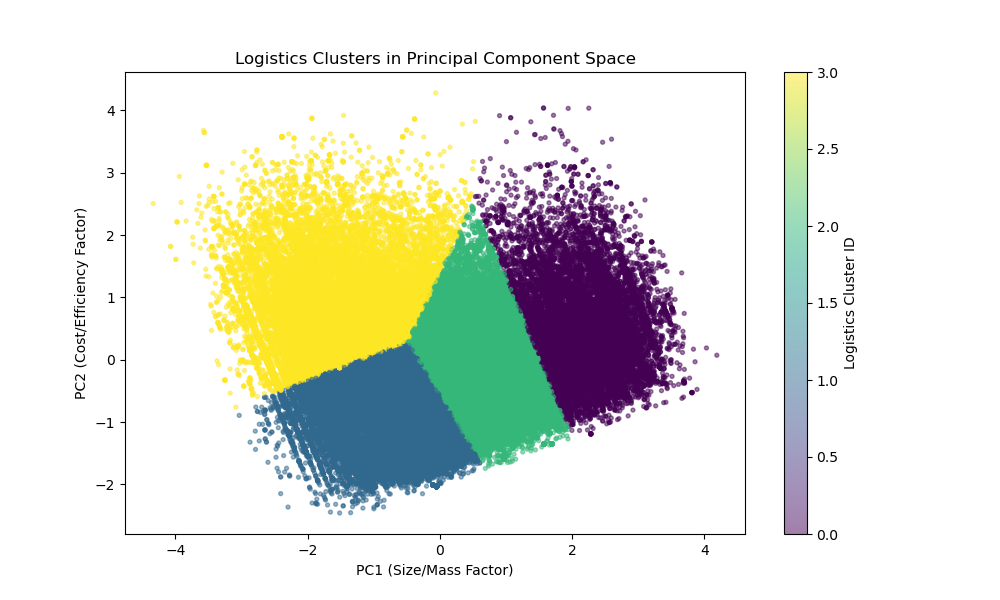
\includegraphics[width=\textwidth]{Figure_1.png}
        \caption{Correlation heatmap identifying primary drivers of bad reviews.}
        \label{fig:correlation}
    \end{minipage}\hfill
    \begin{minipage}{0.48\textwidth}
        \centering
        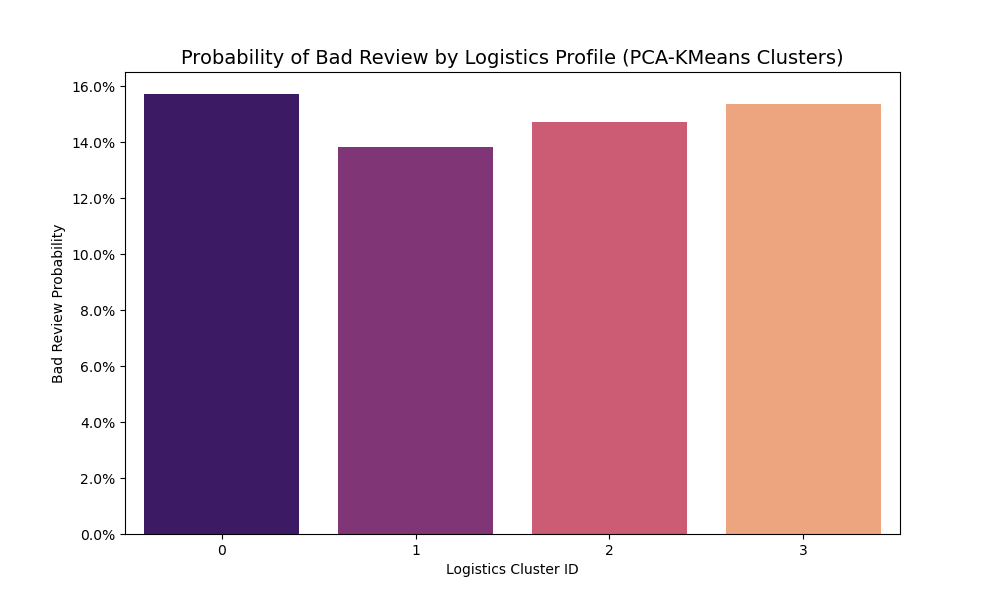
\includegraphics[width=\textwidth]{Figure_2.png}
        \caption{Delivery days vs.\ review score: temporal impact on satisfaction.}
        \label{fig:delivery_box}
    \end{minipage}
\end{figure}

As shown in Figure~\ref{fig:correlation}, \texttt{delay\_days} and \texttt{delivery\_days} exhibit the highest positive correlation with \texttt{is\_bad\_review}, confirming that logistics performance is the primary catalyst for low ratings. Figure~\ref{fig:delivery_box} further illustrates this relationship: 1-star reviews are associated with a significantly higher median delivery time compared to 5-star reviews.

\begin{figure}[H]
    \centering
    \begin{minipage}{0.48\textwidth}
        \centering
        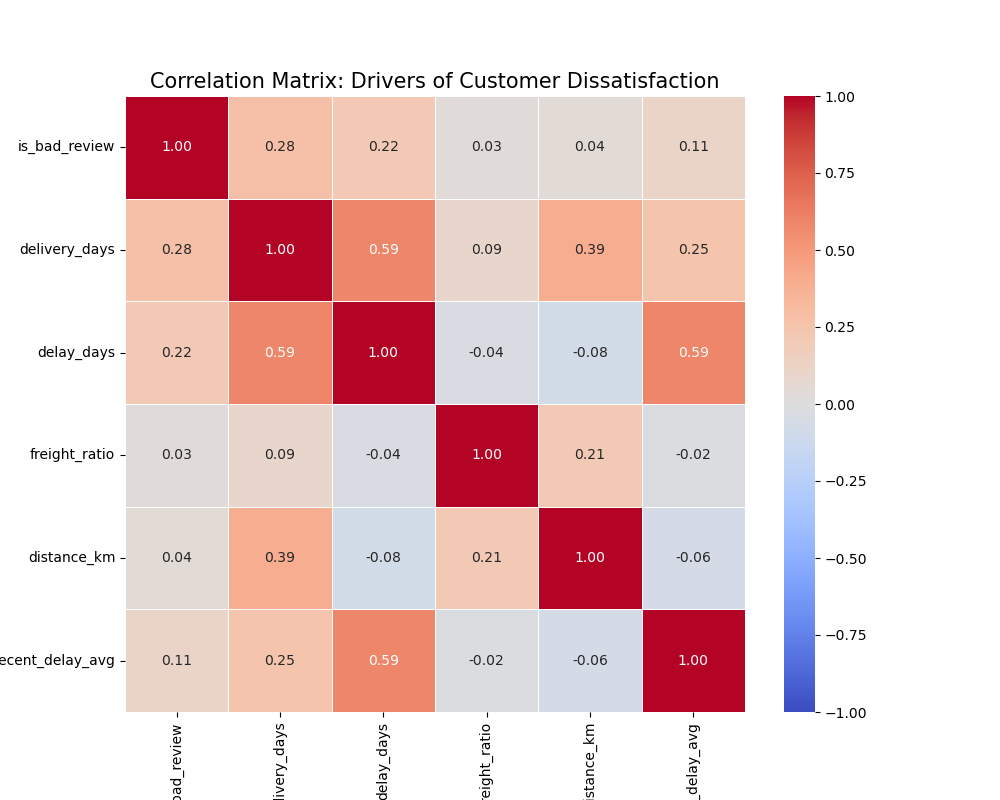
\includegraphics[width=\textwidth]{Figure_3.png}
        \caption{Violin plot of freight ratio across review categories.}
        \label{fig:freight_violin}
    \end{minipage}\hfill
    \begin{minipage}{0.48\textwidth}
        \centering
        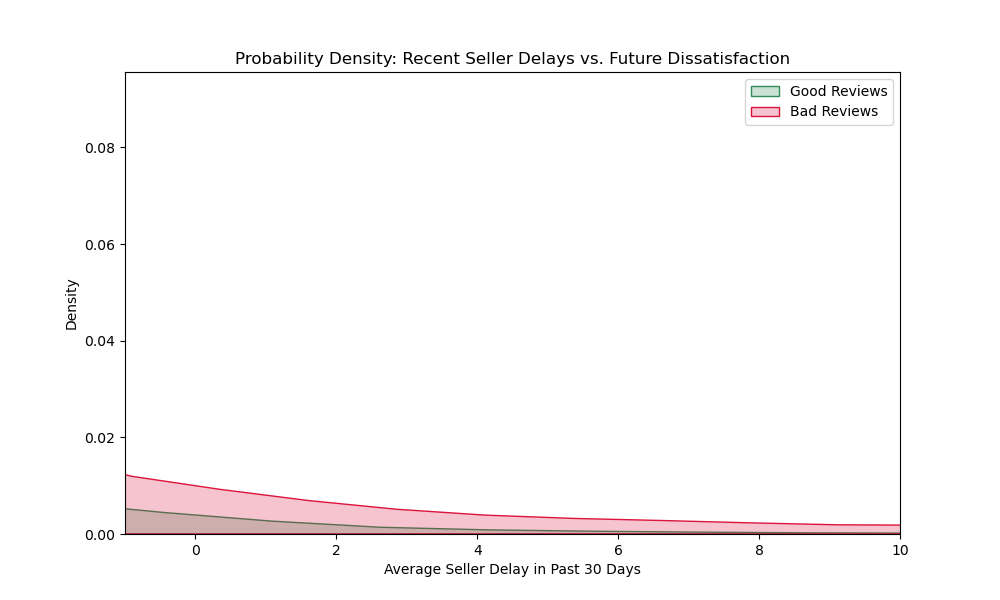
\includegraphics[width=\textwidth]{Figure_6.png}
        \caption{KDE density of the seller's 30-day delay average by review outcome.}
        \label{fig:seller_kde}
    \end{minipage}
\end{figure}

Financial factors also play a critical role. Figure~\ref{fig:freight_violin} reveals that bad reviews are concentrated in the upper quartile of \texttt{freight\_ratio}, identifying the ``freight assassin'' phenomenon where shipping costs exceed item value. Our engineered dynamic feature---the seller's 30-day rolling delay average---shows a distinct heavy tail for bad reviews in Figure~\ref{fig:seller_kde}, validating its use as a predictive signal.

Through these visualizations, we identified that \texttt{delay\_days} (delivery time exceeding the estimated date) is the strongest single continuous driver of bad reviews. Customers are highly sensitive to broken fulfillment promises. Furthermore, evaluating the financial impact via the \texttt{freight\_ratio} revealed that orders with disproportionately high shipping costs suffer from significantly elevated bad-review rates. These insights justified prioritizing temporal tracking and cost-structure features in our predictive pipeline.

\section{Unsupervised Learning}

To discover latent logistics patterns and create additional features for supervised models, we applied a PCA--KMeans pipeline. We first applied a $\log(1+x)$ transformation to skewed physical and cost features to reduce the influence of outliers, then used Principal Component Analysis (PCA) to reduce dimensionality and mitigate noise before clustering.

\begin{figure}[H]
    \centering
    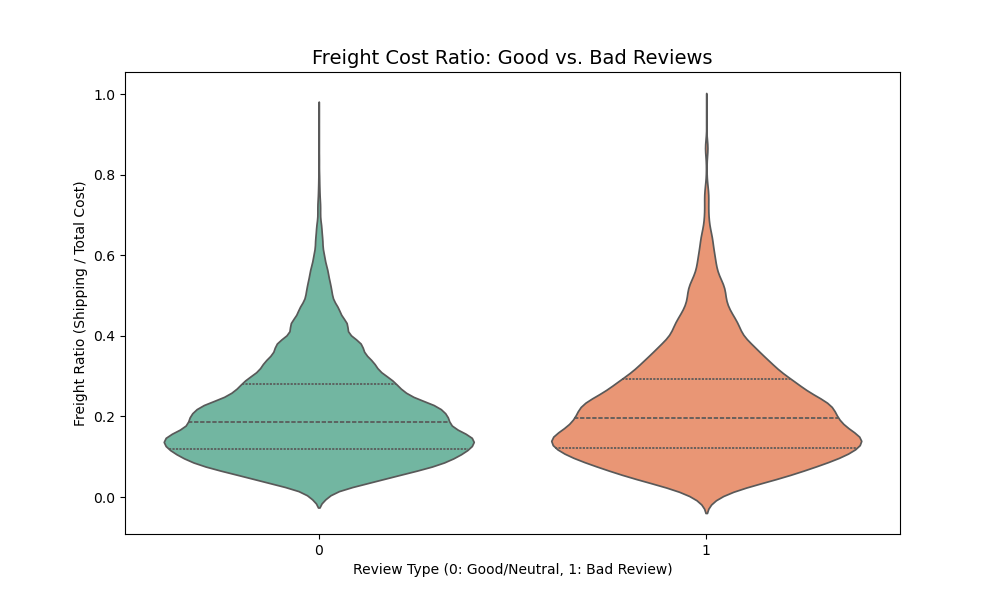
\includegraphics[width=0.75\textwidth]{Figure_5.png}
    \caption{Logistics clusters in PCA space. Four distinct clusters are identified based on product size, weight, and freight efficiency.}
    \label{fig:pca_clusters}
\end{figure}

As visualized in Figure~\ref{fig:pca_clusters}, the K-Means algorithm ($k=4$, chosen by elbow analysis on within-cluster sum of squares) successfully partitioned orders into distinct clusters in the 2D PCA space. To validate the business utility of these clusters, we calculated the probability of bad reviews for each group.

\begin{figure}[H]
    \centering
    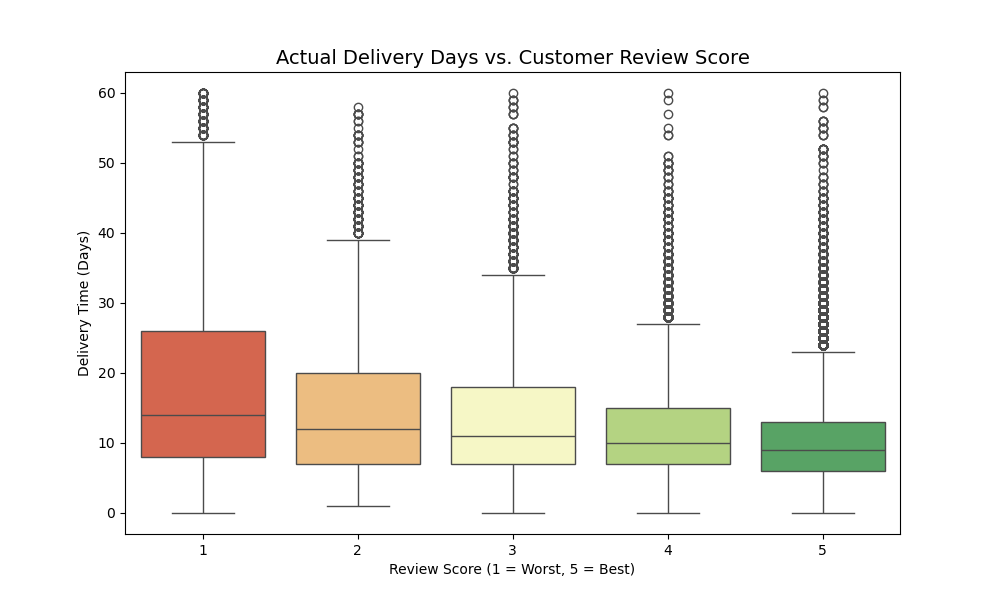
\includegraphics[width=0.75\textwidth]{Figure_4.png}
    \caption{Risk profiling: probability of bad reviews by logistics cluster. Clusters differ significantly in operational risk.}
    \label{fig:cluster_risk}
\end{figure}

Figure~\ref{fig:cluster_risk} demonstrates that the clusters are not just geometric partitions but represent varying levels of operational risk. Clusters associated with heavy or bulky goods or high freight-to-price ratios show a substantially higher propensity for customer dissatisfaction. This confirms that the cluster labels capture meaningful structure beyond what is directly expressed by individual features, justifying their inclusion as categorical features in the supervised models.

\section{Feature Engineering and Preprocessing}

Building on our EDA and unsupervised learning findings, we engineered several advanced features to capture nonlinear business dynamics.

\paragraph{Spatial features.}
We calculated the true spherical distance between buyers and sellers using the Haversine formula, which more accurately reflects logistical difficulty across Brazil's vast geography than a simple Euclidean approximation of latitude--longitude coordinates.

\paragraph{Temporal features.}
We engineered a 30-day dynamic rolling window to calculate each seller's recent average delay. This feature captures real-time seller reliability and short-term operational strain, providing a stronger predictive signal than static historical averages that may be dominated by older, less relevant orders.

\paragraph{Missing value imputation.}
Product dimension records with partial missingness (weight, length, height, width) were imputed using a K-Nearest Neighbors (KNN) imputer fitted on the training partition. KNN imputation preserves the multi-dimensional covariance structure between product dimensions better than mean imputation.

\paragraph{Outlier detection.}
To protect model decision boundaries from noise, we used an Isolation Forest (contamination $= 0.01$) to detect high-dimensional multivariate outliers.

\begin{figure}[H]
    \centering
    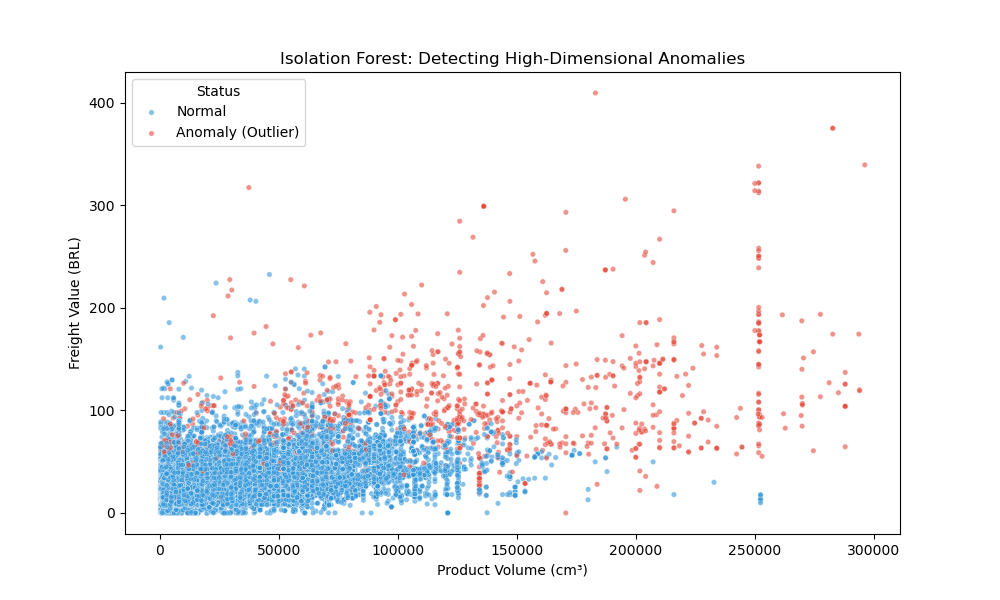
\includegraphics[width=0.75\textwidth]{Figure_7.png}
    \caption{Isolation Forest anomaly detection. Red points represent logical paradoxes in the high-dimensional feature space (e.g., large volume combined with near-zero freight value).}
    \label{fig:isolation_forest}
\end{figure}

As illustrated in Figure~\ref{fig:isolation_forest}, while the vast majority of orders cluster within expected operational bounds, a fraction of the data exhibits logical paradoxes that traditional univariate trimming cannot capture. Removing these isolated anomalies prevents the models from overfitting to recording errors.

\paragraph{Scaling and encoding.}
E-commerce metrics inherently operate on vastly different scales (e.g., delivery delays measured in days versus shipping distances spanning thousands of kilometers).

\begin{figure}[H]
    \centering
    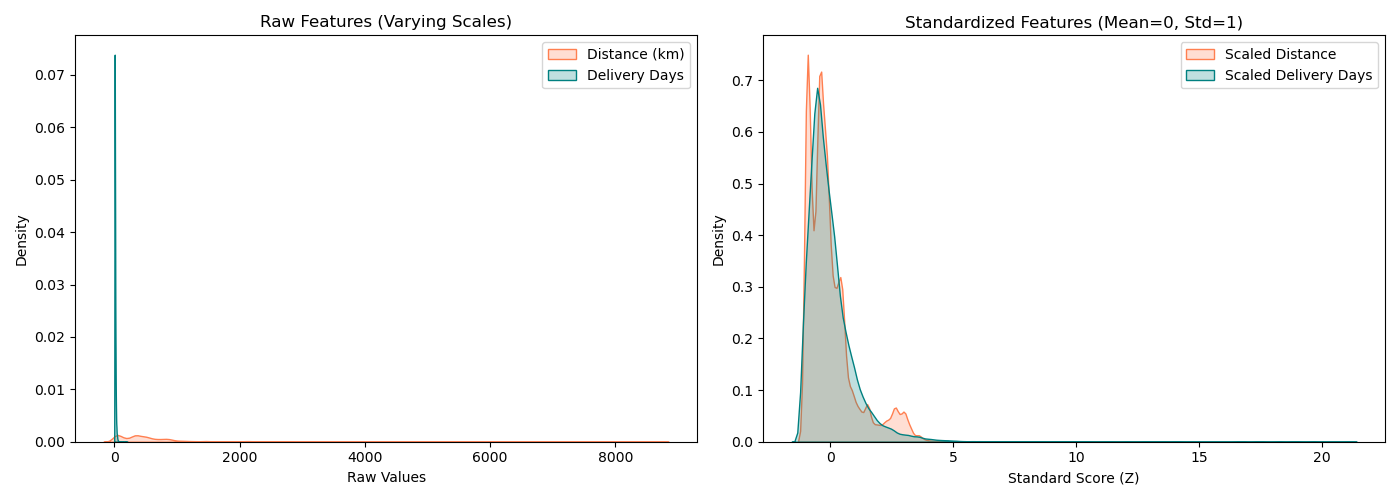
\includegraphics[width=0.9\textwidth]{Figure_8.png}
    \caption{Impact of feature scaling. Left: raw features exhibit extreme variance in scale. Right: \texttt{StandardScaler} aligns features to zero mean and unit variance.}
    \label{fig:feature_scaling}
\end{figure}

Figure~\ref{fig:feature_scaling} demonstrates the necessity of our scaling strategy. Without standardizing, gradient-based models such as logistic regression or the neural network would disproportionately weight features with large numerical magnitudes (e.g., distance in km). By applying \texttt{StandardScaler} (fitted on training data only, applied to all splits), all numeric features are aligned to a standard normal distribution. Categorical features---including seller state, customer state, product category, and the unsupervised logistics cluster labels---were one-hot encoded, yielding a clean, robust, and leakage-free feature matrix.

\section{Supervised Models}

\subsection{Logistic Regression}
\label{sec:lr}

As a baseline model, we trained an L2-regularized logistic regression classifier to predict whether an order would receive a bad review (1--3 stars). Given the class imbalance in the target variable (approximately 15\% bad reviews versus 85\% good reviews), we applied \texttt{class\_weight=balanced} to re-weight the loss function in proportion to class frequencies.

The model was trained on a stratified 80/20 train-test split and validated using 5-fold stratified cross-validation. In total, 135 features were used, comprising 13 standardized numeric features, 3 unsupervised cluster labels derived from the EDA stage, and one-hot encoded customer state, seller state, and product category variables.

\paragraph{Performance.}

The model achieved a ROC-AUC of 0.725 on the held-out test set. Cross-validation produced a mean AUC of 0.714 ($\pm$ 0.007), confirming that performance is stable across data splits and that the model does not overfit.

Overall accuracy was 73.3\%, though this metric is less informative under class imbalance. The F1 score on the bad-review class was 0.391. Recall reached 0.58, meaning the model successfully identified the majority of actual bad reviews, while precision was 0.29, indicating a substantial number of false positives.

This trade-off is expected given the balanced weighting strategy, which lowers the effective decision threshold for the minority class at the cost of increased false positives.

\paragraph{Feature importance.}

Inspection of the model coefficients reveals that \texttt{delivery\_days} was the most influential predictor, with coefficient $+0.683$, approximately 1.7 times larger than any other feature. This indicates that total customer waiting time is more strongly associated with dissatisfaction than whether the order was technically late.

The coefficient for \texttt{delay\_days} was comparatively modest at $+0.065$. The number of items in an order (\texttt{order\_item\_id}, coefficient $= +0.413$) was the second strongest positive predictor, likely reflecting increased fulfillment complexity.

Several product categories, including \texttt{beleza\_saude} ($-0.118$) and \texttt{esporte\_lazer} ($-0.102$), showed negative coefficients, implying lower baseline bad-review rates in these segments.

\paragraph{Limitations.}

Despite its interpretability advantages, logistic regression is constrained to a linear decision boundary and cannot capture feature interactions. For example, it may miss the compounding risk of a heavy product shipped over a long distance by a recently underperforming seller.

The relatively low precision (0.29) suggests that the classification problem contains meaningful nonlinear structure, motivating more expressive models in the following sections.

\subsection{Gradient-Boosted Trees}
\label{sec:gbt}

To capture nonlinear relationships and interactions among features, we trained a Gradient-Boosted Trees (GBT) classifier as a more expressive alternative to logistic regression. Gradient boosting builds an ensemble of decision trees sequentially, where each tree is trained to correct the residuals of the previous ones, enabling the model to capture complex patterns that a single linear boundary cannot.

The model was trained using the same stratified 80/20 train-test split as the baseline model to ensure a fair comparison, and the same feature set was used. Hyperparameter tuning was performed via grid search over the number of estimators, learning rate, and maximum tree depth.

\paragraph{Performance.}

\begin{table}[H]
\centering
\caption{Gradient-boosted trees evaluation on the held-out test set.}
\label{tab:gbt_results}
\begin{tabular}{lc}
\toprule
Metric & Value \\
\midrule
Accuracy  & 91.5\% \\
Precision & 1.000  \\
Recall    & 0.633  \\
F1 Score  & 0.775  \\
ROC-AUC   & 0.861  \\
\bottomrule
\end{tabular}
\end{table}

The GBT model achieved a ROC-AUC of 0.861 on the held-out test set (Table~\ref{tab:gbt_results}), representing a substantial improvement over the logistic regression baseline (AUC 0.725). The ROC curve confirms that the model maintains a high true positive rate across different operating thresholds.

The precision of 1.000 at the default decision threshold indicates that every order flagged as a bad review by the model was indeed a bad review, at the cost of recall (0.633): a substantial fraction of actual bad reviews were not caught. Depending on the operational context, the threshold can be lowered to increase recall.

\paragraph{Feature importance.}

Feature importance analysis reveals that temporal features---\texttt{delivery\_days} and \texttt{delay\_days}---are among the most influential predictors, consistent with the EDA findings. The cluster labels from the unsupervised pipeline also contribute meaningfully, confirming that the latent logistics structure captured by KMeans adds signal beyond the raw numeric features. Unlike logistic regression, the GBT model captures interactions between these features automatically.

\paragraph{Advantages over logistic regression.}

The GBT model's key advantage is its ability to model nonlinear patterns and feature interactions. The improvement in AUC from 0.725 to 0.861 demonstrates that the underlying prediction task contains meaningful nonlinear structure. Additionally, GBT is robust to feature scale differences without requiring explicit normalization.

\subsection{Feed-Forward Neural Network}
\label{sec:dnn}

A feed-forward multilayer perceptron (MLP) was trained as an \textit{ordinal-regularized multi-class classifier} over \texttt{review\_score} $\in \{1,2,3,4,5\}$. The target is not truly continuous: it is an ordered set of five discrete categories, and a regression formulation is drawn toward the modal class (5$\star$, 57.5\% of orders), compressing all predictions toward the mean. A classification head produces a full probability distribution over the five classes, giving the model structural freedom to assign high probability to extreme ratings when the evidence supports it.

A note on terminology: this model uses a standard five-class softmax output rather than a true ordinal threshold architecture such as CORAL or CORN, which encode monotone cumulative probabilities by construction. Ordinal structure is instead enforced through the loss function, described below.

\paragraph{Feature pipeline.}
The feature matrix was constructed from \texttt{clean\_df\_final.csv} (108{,}911 rows). All identifier, timestamp, and city/zip columns were dropped along with the derived column \texttt{is\_bad\_review}. The remaining columns were partitioned into three groups.
\begin{itemize}[noitemsep]
  \item \textbf{Numeric} (22 columns): price, freight, distances, delays, product dimensions, cluster indicators, and coordinates. Median imputation (fitted on the training partition) was applied to residual missing values; a fresh \texttt{StandardScaler}, also fitted on training data only, standardized these columns before each training run.
  \item \textbf{One-hot encoded} (49 columns): \texttt{seller\_state} (22 levels) and \texttt{customer\_state} (27 levels).
  \item \textbf{Embedding} (8 dimensions): \texttt{product\_category\_name} (74 categories, including an \texttt{unknown} level for unseen categories at inference) was mapped to a learned 8-dimensional embedding via \texttt{nn.Embedding}.
\end{itemize}
The 22 numeric and 49 OHE columns form a 71-dimensional dense vector; concatenating the 8-dimensional embedding gives a 79-dimensional input to the first hidden layer.

\paragraph{Architecture.}
Each candidate MLP follows the block structure
\[
\bigl[\mathbf{x}_{\mathrm{dense}},\;\mathrm{Emb}(c)\bigr]
\;\longrightarrow\;
\bigl[\,\mathrm{Linear} \to \mathrm{BatchNorm} \to \mathrm{Act} \to \mathrm{Dropout}\,\bigr]^{L}
\;\longrightarrow\;
\mathrm{Linear}(5),
\]
where $\mathbf{x}_{\mathrm{dense}} \in \mathbb{R}^{71}$, $\mathrm{Emb}(c) \in \mathbb{R}^{8}$, and $L$ hidden layers each have uniform width $d$. Batch normalization stabilizes gradient flow; dropout regularizes. The output layer produces five raw logits---one per star rating---with no final activation. At inference time, the predicted class is $\mathrm{argmax}(\mathrm{logits}) + 1 \in \{1,\dots,5\}$.

\paragraph{Loss function.}
Training minimized a combined ordinal loss:
\[
\mathcal{L}
= \underbrace{\mathrm{CE}_{\mathrm{w}}(\mathbf{p}, y)}_{\text{class-weighted CE}}
+ \;\lambda\;\underbrace{\Bigl(\sum_{k=1}^{5} k\,\hat{p}_k - y\Bigr)^{\!2}}_{\text{ordinal MSE}},
\quad \lambda = 0.5,
\]
where $\hat{p}_k = \mathrm{softmax}(\mathrm{logits})_k$ and $y \in \{1,\dots,5\}$ is the true score.

The cross-entropy term uses inverse-frequency class weights to counteract the severe imbalance: $w_k = N / (5 \cdot n_k)$, yielding $w_2 \approx 5.96$ for the rarest class and $w_5 \approx 0.35$ for the most common. The ordinal MSE term penalizes mispredictions proportionally to their distance from the true class in expectation, so predicting 5$\star$ for a 1$\star$ order incurs a larger penalty than predicting 2$\star$. The two terms address orthogonal problems: class weights correct imbalance; the ordinal term encodes the ordering structure.

Early stopping monitored the held-out validation combined loss with a patience of 10 epochs, restoring the best-weight checkpoint; maximum epoch budget was 100.

\paragraph{Hyperparameter search.}
Bayesian optimization via Optuna's TPE sampler was used. A MedianPruner discarded unpromising trials after two warm-up folds. Each trial was evaluated on 5-fold \texttt{StratifiedKFold} cross-validation (each fold preserving the 1$\star$--5$\star$ class distribution); the objective was mean fold validation combined loss. To prevent leakage, all preprocessing was fold-local: one-hot encoding, median imputation, the product-category embedding vocabulary, and the feature scaler were all fitted on the fold's training partition only. Product categories appearing only in a validation fold received the reserved \texttt{unknown} embedding, so no validation-row information influenced any preprocessing step. Twenty trials were run on CPU. The search space is summarized in Table~\ref{tab:dnn_search}.

\begin{table}[H]
\centering
\caption{MLP hyperparameter search space.}
\label{tab:dnn_search}
\begin{tabular}{lll}
\toprule
Parameter & Type & Range / Choices \\
\midrule
Number of hidden layers ($L$) & Integer          & 2--5 \\
Hidden layer width ($d$)       & Integer (log)    & 64--512 \\
Dropout rate                   & Float            & 0.0--0.5 \\
Learning rate                  & Float (log)      & $10^{-4}$--$10^{-2}$ \\
Weight decay                   & Float (log)      & $10^{-5}$--$10^{-2}$ \\
Batch size                     & Categorical      & \{1024, 2048, 4096\} \\
Activation function            & Categorical      & \{ReLU, GELU, ELU\} \\
\bottomrule
\end{tabular}
\end{table}

\paragraph{Final training and evaluation.}
The best trial's configuration was retrained from scratch on a stratified 90\% subset of the 80\% training partition, with the remaining 10\% used as an internal early-stopping validation set. The locked 20\% test set was used only for the single final evaluation. Metrics reported are overall accuracy, mean absolute error on predicted class (MAE, interpretable as average stars off), and quadratic weighted kappa (QWK), which penalizes distant misclassifications more heavily and is a standard metric for ordinal classification.

\paragraph{Results.}
Test-set performance is reported in Table~\ref{tab:dnn_results}. Per-class accuracy and the row-normalised confusion matrix are shown in Figure~\ref{fig:dnn_per_score}.

\begin{table}[H]
\centering
\caption{DNN ordinal classifier evaluation on the held-out test set (21{,}783 orders).}
\label{tab:dnn_results}
\begin{tabular}{lcc}
\toprule
Metric & CV (search) & Test \\
\midrule
Combined loss (CE + $\lambda$ ordinal MSE) & 2.4548 & --- \\
Accuracy           & ---    & 57.98\% \\
MAE (stars off)    & ---    & 0.825 \\
QWK                & ---    & 0.338 \\
\bottomrule
\end{tabular}
\end{table}

The best trial (trial 17 of 20) used 3 hidden layers of width 226, ReLU activations, dropout 0.272, learning rate $1.65 \times 10^{-3}$, weight decay $7.0 \times 10^{-5}$, and batch size 2048.

Per-class accuracy on the test set reveals that the model concentrates most of its probability mass on the 5$\star$ class: accuracy is 92.6\% for true 5$\star$ orders but only 29.6\%, 9.8\%, 7.9\%, and 1.7\% for 1$\star$ through 4$\star$ respectively. Overall accuracy of 57.98\% matches the 5$\star$ base rate, and QWK of 0.338 (``fair'' agreement) reflects meaningful signal above chance but substantial room for improvement. Addressing the residual majority-class collapse---for instance via stronger class weights, a true ordinal threshold architecture, or oversampling of minority ratings---is an avenue for future work.

\begin{figure}[H]
\centering
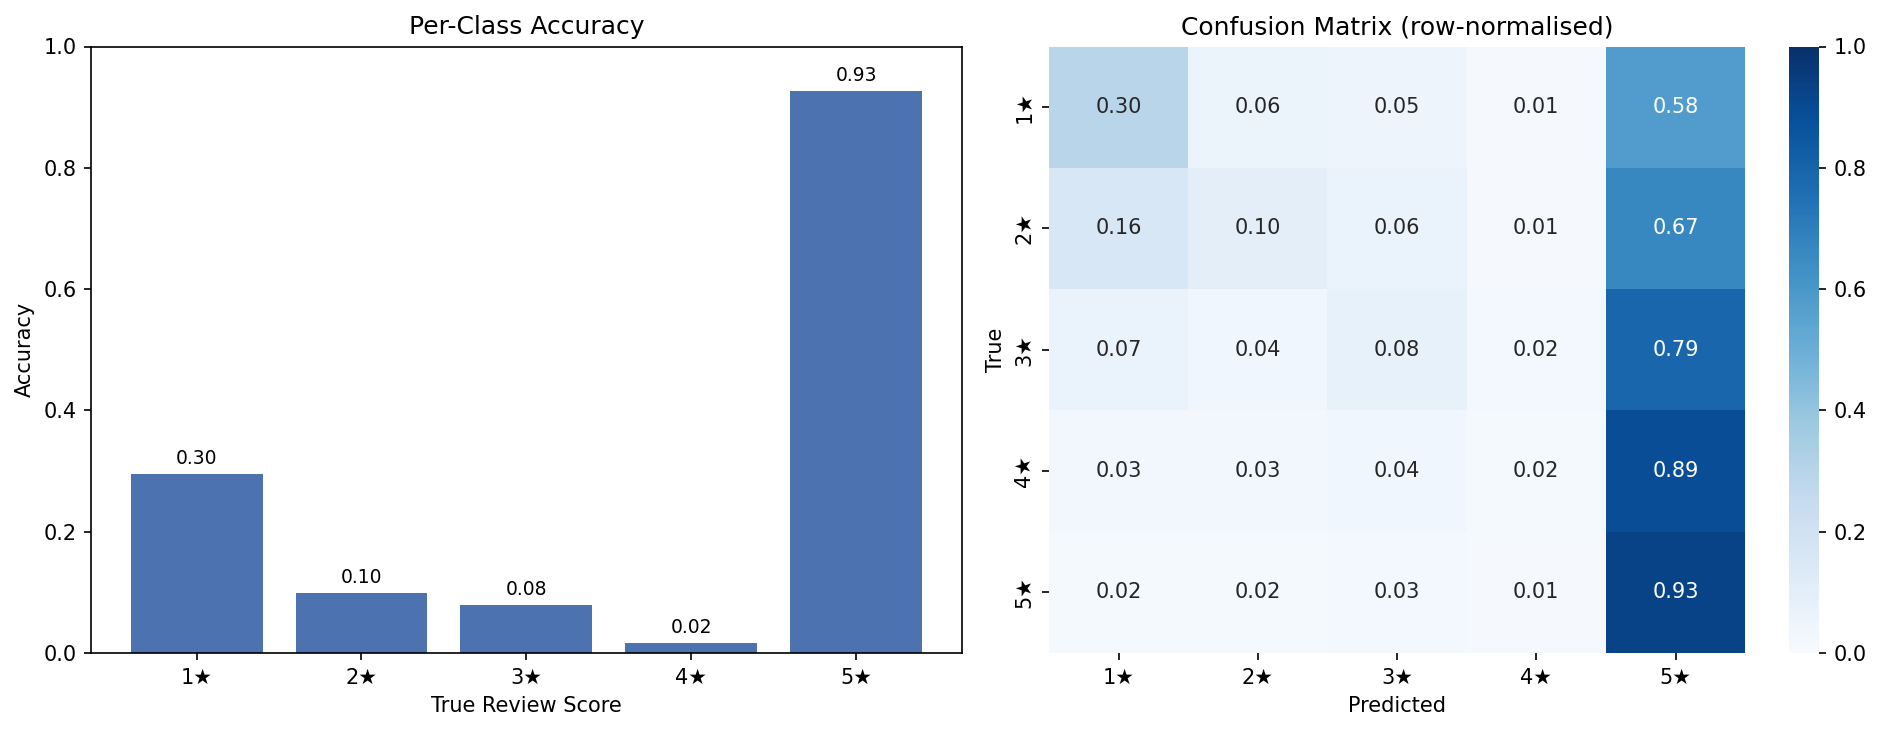
\includegraphics[width=0.9\textwidth]{../figures/dnn_per_score.png}
\caption{Left: per-class accuracy by true star rating. Right: row-normalised confusion matrix. Both from the held-out test set.}
\label{fig:dnn_per_score}
\end{figure}

\section{Model Comparison and Final Selection}

\paragraph{Framing.}
The three models operate on related but not identical formulations. Logistic regression and gradient-boosted trees solve a binary classification task (bad review: \texttt{review\_score} $\leq 3$ vs.\ good review), which is the most operationally actionable framing. The DNN solves the harder five-class ordinal task. Direct metric comparison is therefore informative but should be interpreted with this framing difference in mind.

\paragraph{Summary of results.}

\begin{table}[H]
\centering
\caption{Model comparison on the held-out test set. LR and GBT report binary bad-review metrics; DNN reports ordinal five-class metrics.}
\label{tab:comparison}
\begin{tabular}{lccccc}
\toprule
Model & Task & ROC-AUC & Accuracy & F1 / QWK & Recall \\
\midrule
Logistic Regression & Binary & 0.725 & 73.3\% & F1 = 0.391 & 0.58 \\
Gradient-Boosted Trees & Binary & 0.861 & 91.5\% & F1 = 0.775 & 0.633 \\
Feed-Forward Neural Network & 5-class ordinal & --- & 57.98\% & QWK = 0.338 & --- \\
\bottomrule
\end{tabular}
\end{table}

\paragraph{Interpretability.}
Logistic regression offers the clearest interpretability: individual feature coefficients directly quantify the marginal contribution of each variable. The GBT model is less directly interpretable but supports feature importance rankings and partial dependence plots. The DNN is the least interpretable of the three, though the learned product-category embeddings can be visualized geometrically.

\paragraph{Final model selection.}
For the binary bad-review prediction task, \textbf{gradient-boosted trees} is selected as the preferred model. It achieves the highest ROC-AUC (0.861 vs.\ 0.725 for logistic regression) and F1 score (0.775), demonstrating that the nonlinear feature interactions and automatic handling of feature scale differences provide substantial gains over the linear baseline. Its performance is robust across the held-out test set, and the decision threshold can be adjusted to trade precision for recall depending on operational priorities.

The neural network is recommended for the full five-class ordinal setting, where predicting the specific star rating---rather than a binary flag---is required. Its QWK of 0.338 represents meaningful signal above chance despite the severe class imbalance, and the ordinal loss formulation is more principled than treating all misclassifications equally.

\section{Discussion}

\paragraph{Key findings.}
The dominant driver of customer dissatisfaction in this dataset is logistics performance, specifically total delivery time (\texttt{delivery\_days}) and delivery delay relative to the estimated date (\texttt{delay\_days}). This finding is consistent across all three models and across the EDA stage. A secondary driver is the freight cost ratio: orders where shipping costs represent an outsized fraction of the item value are significantly more likely to receive bad reviews. These insights suggest that operational interventions---improved logistics routing, more conservative delivery date estimates, or proactive communication during delays---would be more effective than product-side changes for reducing bad reviews at scale.

\paragraph{Modeling tradeoffs.}
The most important tradeoff in this project was between interpretability and predictive capacity. Logistic regression is transparent but misses nonlinear interactions. GBT captures those interactions and nearly doubles the F1 score, at the cost of a less directly interpretable model. The DNN offers the richest representational capacity and the most principled treatment of the ordinal target, but its per-class accuracy is dominated by the modal 5-star class, and its QWK of 0.338 is lower than might be expected for a model of this scale---a consequence of the severe class imbalance that proves difficult to fully overcome even with class weighting and ordinal regularization.

\paragraph{Limitations.}
First, the dataset covers a specific time period and market (Brazil, 2016--2018); generalization to other geographies or time periods should not be assumed. Second, the precision of 1.000 reported for the GBT model at the default threshold is likely an artifact of the threshold value and should not be taken as a guarantee of perfect bad-review identification in deployment. Third, the DNN results show that majority-class collapse remains a challenge even with the ordinal loss formulation; more aggressive resampling or a true ordinal threshold architecture may be needed for production use. Finally, several potentially informative features---seller historical performance beyond 30 days, product return rates, customer tenure---were unavailable or out of scope.

\paragraph{Future work.}
Possible extensions include: (1) applying SHAP values to the GBT model for instance-level explanations, (2) exploring CORAL or CORN architectures for the ordinal classification task, (3) adding time-series features that capture macro-level platform performance trends, and (4) building a real-time scoring API that outputs predicted review risk at the moment of order dispatch.

\section{Reproducibility}

All code is available in the project GitHub repository at \url{https://github.com/FlamyFlame/applied-data-science-project4}. The repository is organized as follows:

\begin{itemize}[noitemsep]
  \item \texttt{data/} --- raw Olist CSV files (downloaded from Kaggle; not committed due to size, but the download script is provided)
  \item \texttt{processed/} --- cleaned and merged analysis-ready CSVs
  \item \texttt{src/} --- model training scripts: \texttt{logistic\_regression.py}, \texttt{gradient\_boosted\_trees.py}
  \item \texttt{notebooks/} --- exploratory notebooks for EDA and unsupervised learning
  \item \texttt{figures/} --- all generated figures
  \item \texttt{reports/} --- this report and supporting output files
  \item \texttt{pipeline.py} --- end-to-end pipeline script (data cleaning through feature engineering)
\end{itemize}

\paragraph{Software environment.}
Python 3.10 was used throughout. Key dependencies: \texttt{pandas} (data manipulation), \texttt{scikit-learn} (logistic regression, GBT, preprocessing, cross-validation), \texttt{PyTorch} (DNN), \texttt{optuna} (Bayesian hyperparameter search), \texttt{matplotlib} and \texttt{seaborn} (visualization). A complete \texttt{requirements.txt} is included in the repository root.

\paragraph{Execution.}
Running \texttt{python pipeline.py} from the repository root reproduces the cleaned dataset. Individual model scripts in \texttt{src/} can then be run to reproduce model training and evaluation results. The DNN training script is deterministic given a fixed random seed (\texttt{seed=42}) set at the top of the file.

\section{Team Contributions}

\begin{itemize}[leftmargin=1.5em]
    \item \textbf{Yuhan Guo:} DNN design and implementation, ordinal loss formulation, Optuna hyperparameter search, leakage prevention audit, report writing (DNN section, model comparison, discussion, reproducibility).
    \item \textbf{Bohong Zheng:} Gradient-boosted trees model, hyperparameter tuning, ROC analysis, GBT feature importance, report writing (GBT section).
    \item \textbf{Xiang Li:} Exploratory data analysis, unsupervised learning (PCA--KMeans pipeline), cluster risk profiling, report writing (EDA and unsupervised sections).
    \item \textbf{Jiahao Wang:} Data acquisition, cleaning and join logic, feature engineering (Haversine distance, rolling seller delay, KNN imputation, Isolation Forest, scaling), logistic regression baseline, report writing (data preparation, feature engineering, LR sections).
\end{itemize}

\section{Conclusion}

This project demonstrated an end-to-end machine learning workflow on the Olist Brazilian e-commerce dataset, from raw multi-table data to a deployed-ready predictive model. The central finding is that logistics performance---particularly total delivery time and delay relative to the promised date---is the dominant driver of customer dissatisfaction, and that this signal is strong enough to support useful prediction before delivery occurs.

Among the three model families evaluated, gradient-boosted trees provided the best performance for the binary bad-review task (ROC-AUC 0.861, F1 0.775), capturing the nonlinear feature interactions that a linear model cannot represent. The DNN with an ordinal-regularized loss addressed the harder five-class formulation and demonstrated that the ordering structure of star ratings can be usefully encoded in the loss function, though majority-class collapse remains a challenge under severe imbalance. Taken together, the models provide complementary perspectives: the GBT is recommended for operational flagging of at-risk orders, while the DNN offers a path toward full review-score prediction.

\begin{thebibliography}{9}

\bibitem{dataset}
Olist. \textit{Brazilian E-Commerce Public Dataset}. Kaggle, 2018. \url{https://www.kaggle.com/datasets/olistbr/brazilian-ecommerce}

\bibitem{friedman2001}
J.\ H.\ Friedman. Greedy function approximation: a gradient boosting machine. \textit{Annals of Statistics}, 29(5):1189--1232, 2001.

\bibitem{coral}
W.\ Cao, V.\ Mirjalili, and S.\ Raschka. Rank consistent ordinal regression for neural networks with application to age estimation. \textit{Pattern Recognition Letters}, 140:325--331, 2020.

\end{thebibliography}

\appendix

\section{Additional Figures}

\begin{figure}[H]
\centering
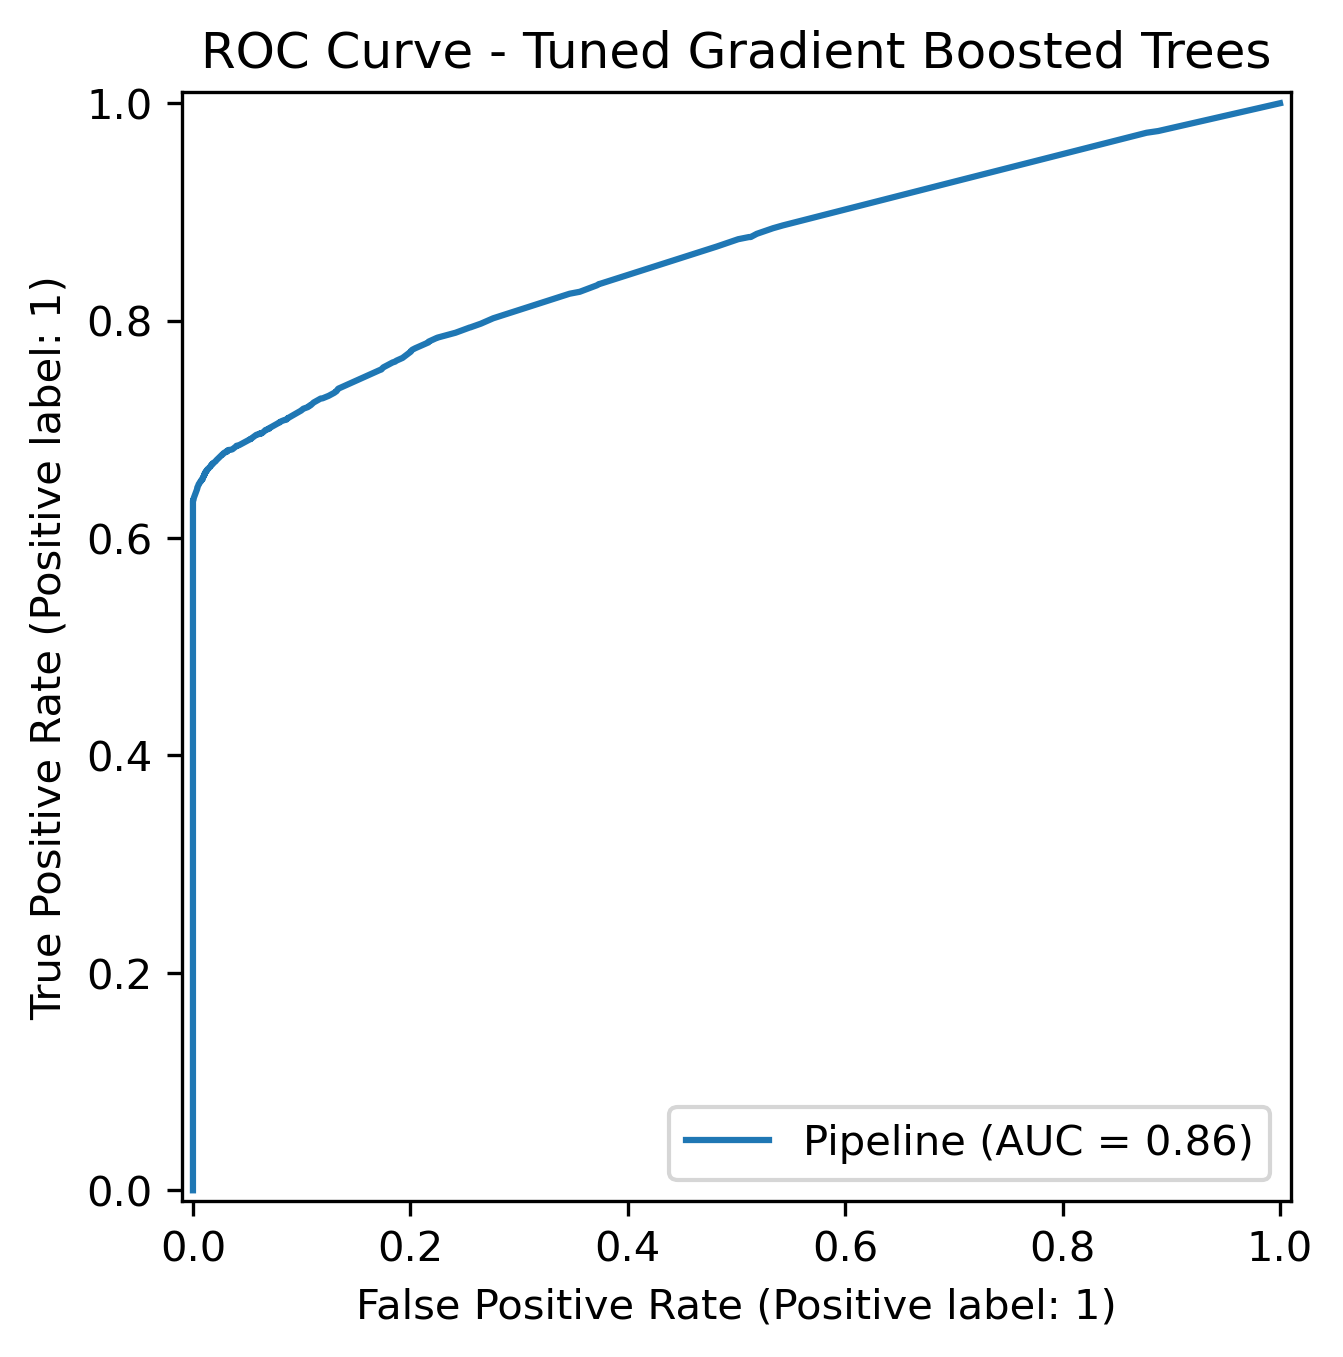
\includegraphics[width=0.7\textwidth]{../figures/roc_curve_tuned_gbt.png}
\caption{ROC curve for the tuned gradient-boosted trees model on the held-out test set (AUC = 0.861).}
\label{fig:gbt_roc}
\end{figure}

\begin{figure}[H]
\centering
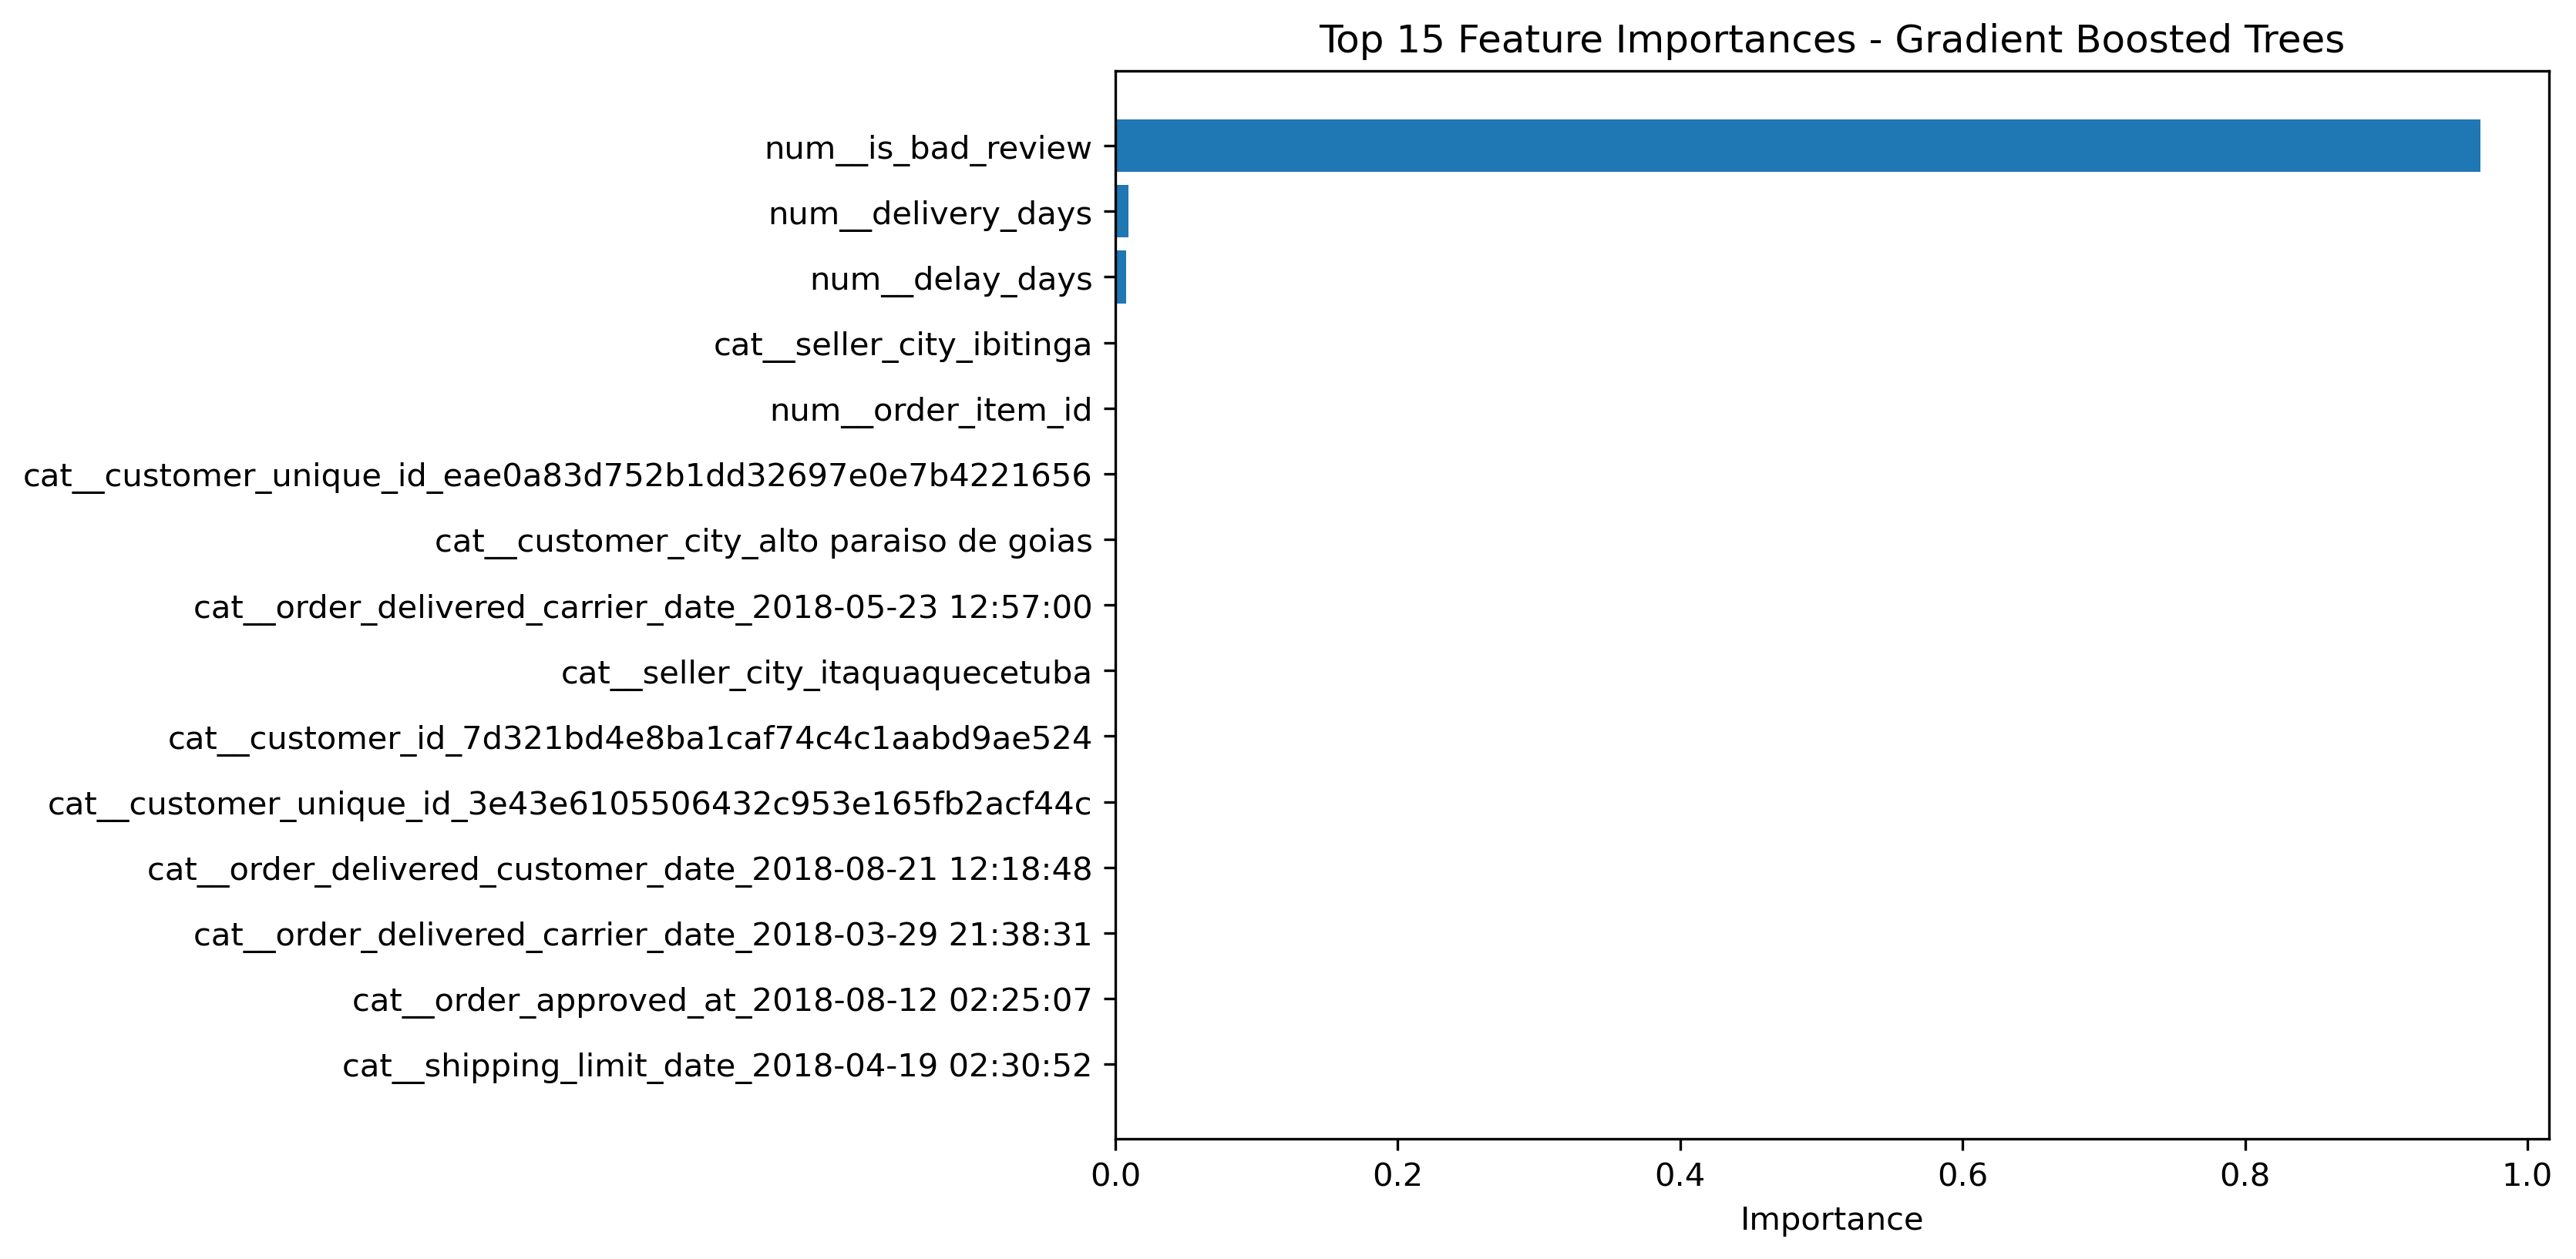
\includegraphics[width=0.7\textwidth]{../figures/feature_importance_gbt.png}
\caption{Top feature importances from the gradient-boosted trees model.}
\label{fig:gbt_fi}
\end{figure}

\begin{figure}[H]
\centering
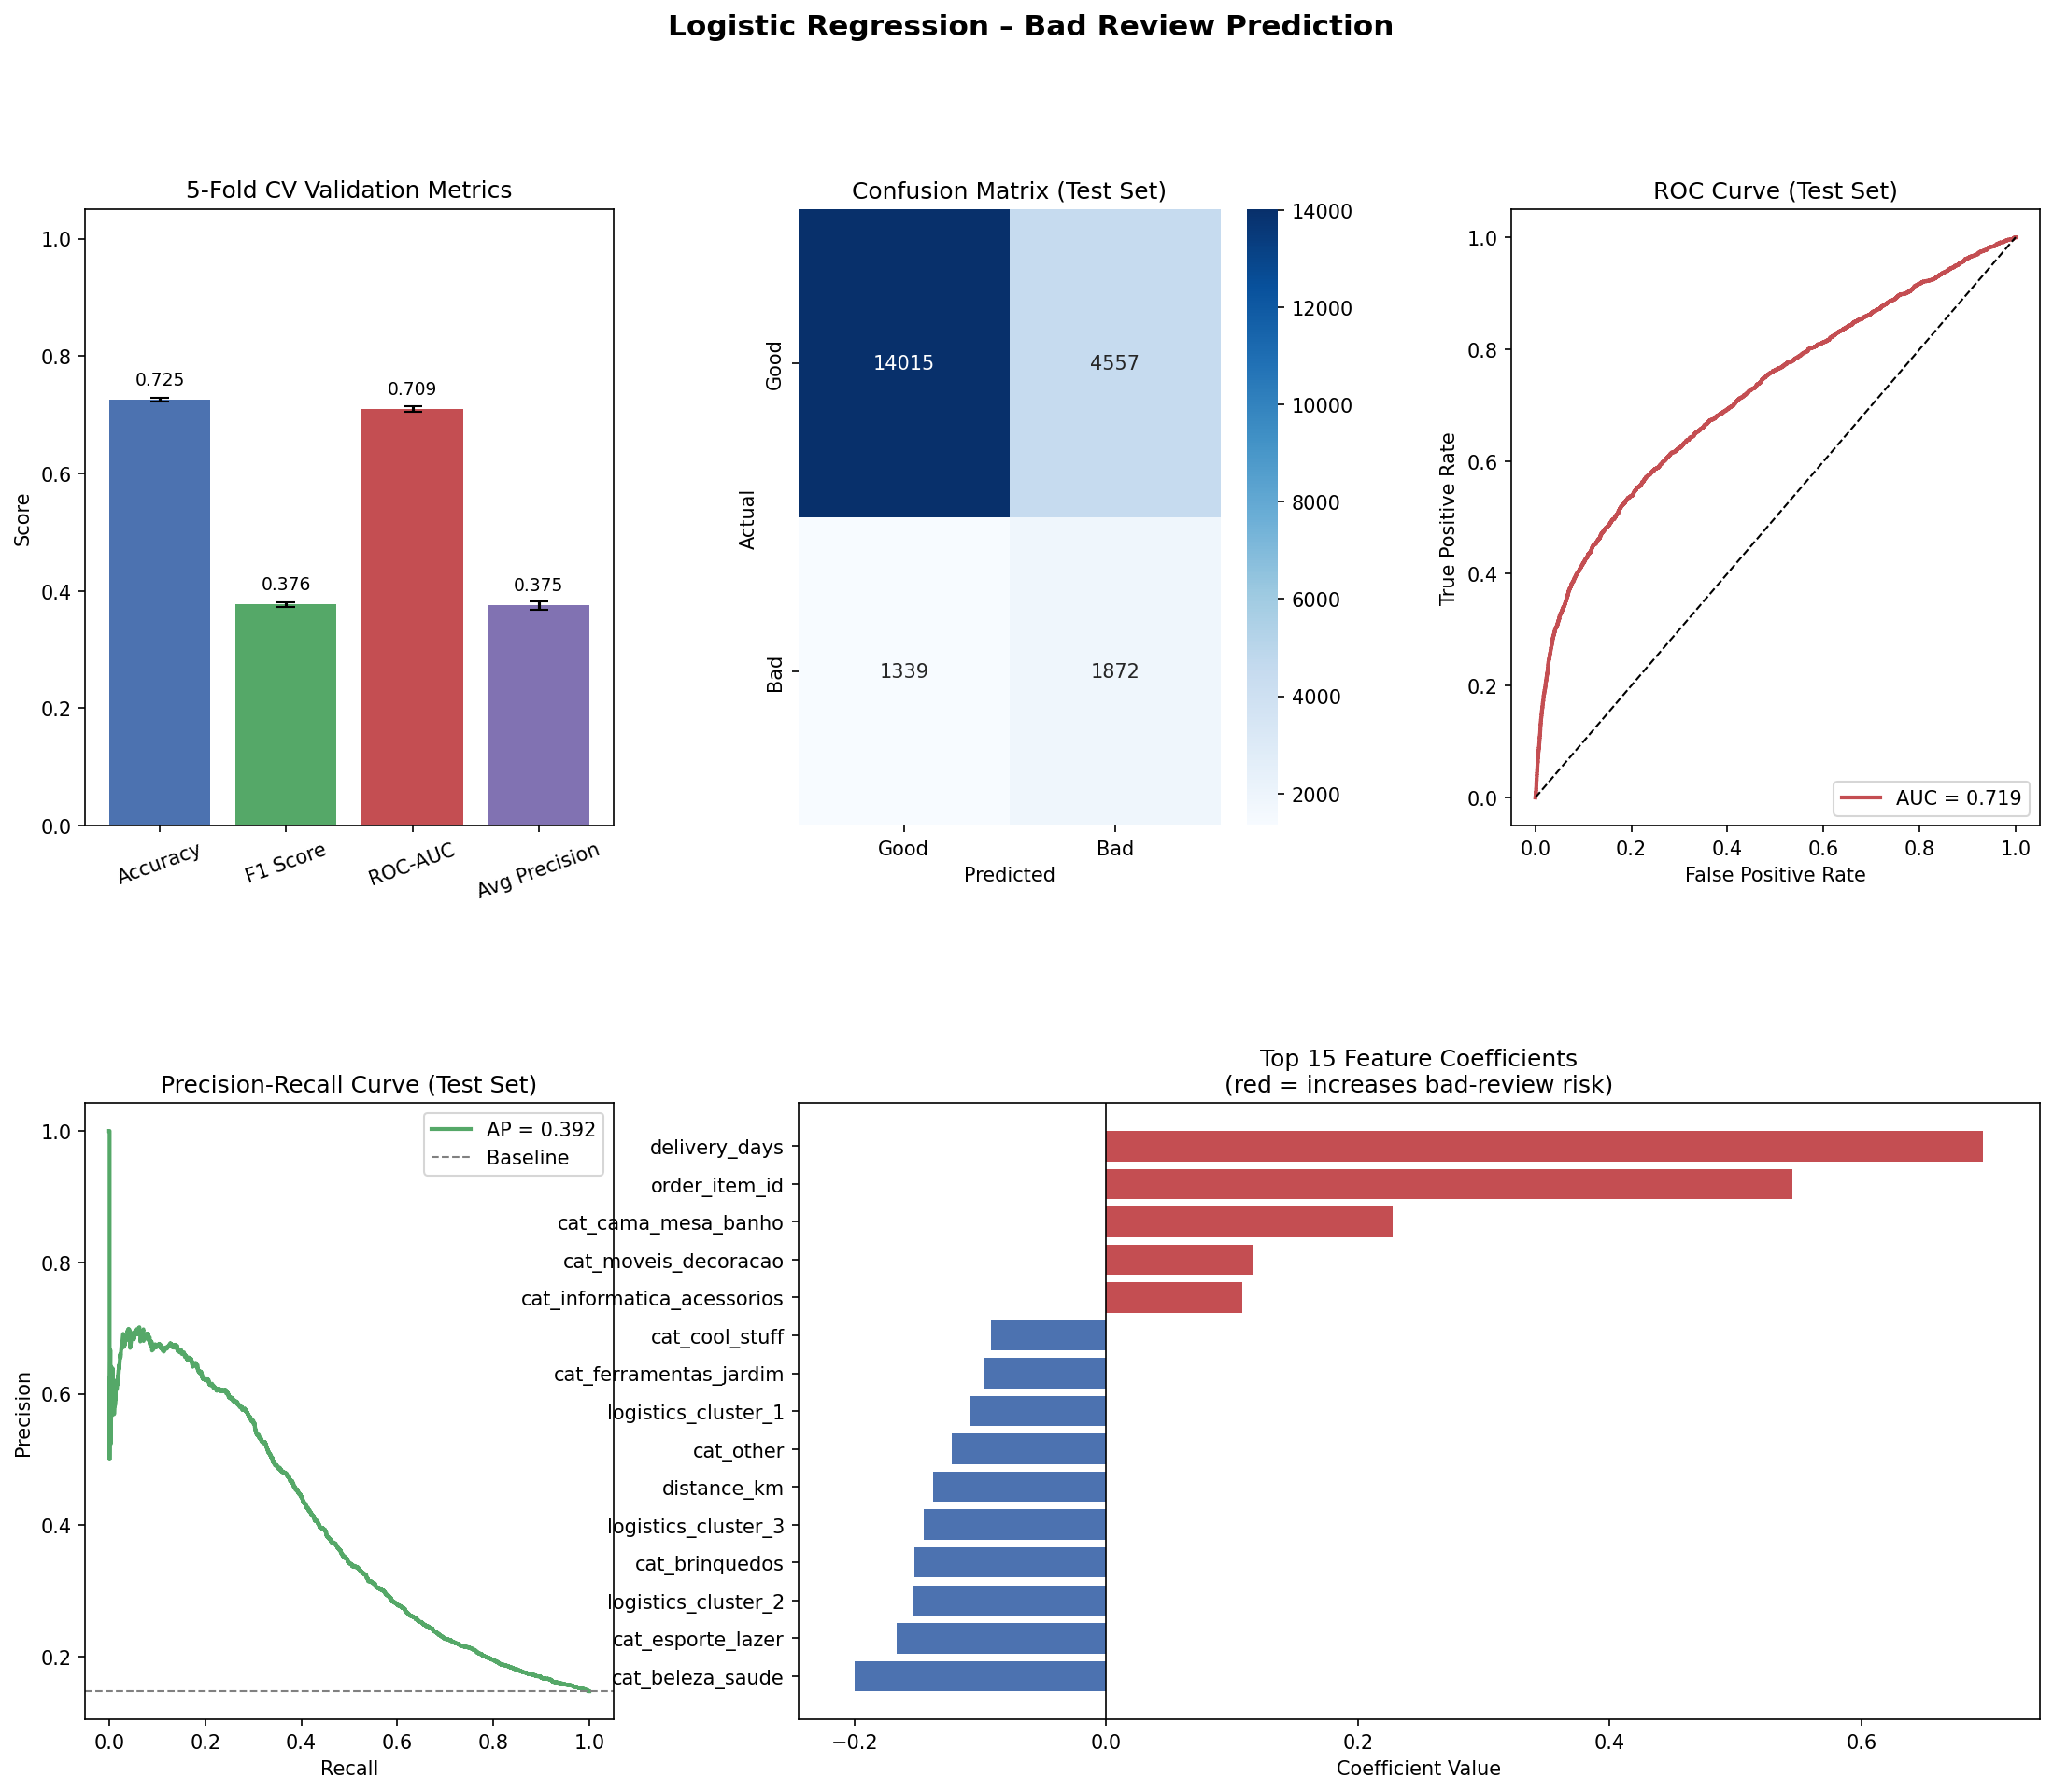
\includegraphics[width=0.7\textwidth]{../figures/logistic_regression_results.png}
\caption{Logistic regression: ROC curve and coefficient bar chart on the held-out test set.}
\label{fig:lr_results}
\end{figure}

\end{document}
